\usetikzlibrary{positioning}
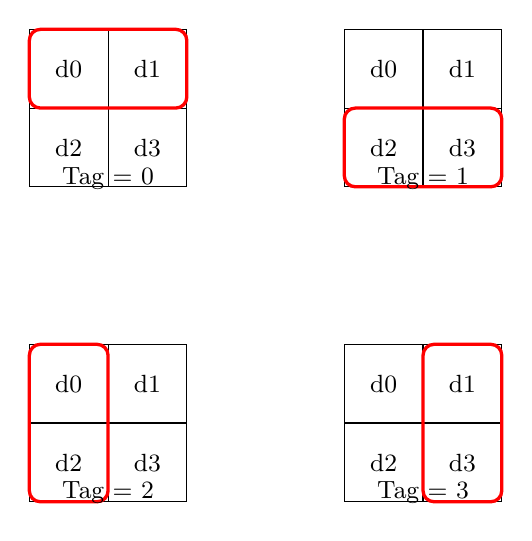
\begin{tikzpicture}[every node/.style={font=\small}]
    % Outer 2x2 grid
    \foreach \i in {0,1} {
        \foreach \j in {0,1} {
            \begin{scope}[shift={(\j*4, -\i*4)}]
                % Inner 2x2 grid
                \draw (0,0) rectangle (2,2);
                \draw (1,0) -- (1,2);
                \draw (0,1) -- (2,1);
                % Label digits
                \node (d\i\j) at (1,1) {}; % For relative positioning
                \node at (0.5,1.5) {d0};
                \node at (1.5,1.5) {d1};
                \node at (0.5,0.5) {d2};
                \node at (1.5,0.5) {d3};
                
                % Highlight depending on program id
                \ifnum\i=0
                    \ifnum\j=0
                        % Program 0: top row (d0, d1)
                        \draw[red,very thick,rounded corners] (0,1) rectangle (2,2);
                    \else
                        % Program 1: bottom row (d2, d3)
                        \draw[red,very thick,rounded corners] (0,0) rectangle (2,1);
                    \fi
                \else
                    \ifnum\j=0
                        % Program 2: left column (d0, d2)
                        \draw[red,very thick,rounded corners] (0,0) rectangle (1,2);
                    \else
                        % Program 3: right column (d1, d3)
                        \draw[red,very thick,rounded corners] (1,0) rectangle (2,2);
                    \fi
                \fi
            \end{scope}
        }
    }

    % Program ID labels relative to grids
    \node[below=0.5cm of d10] {Tag = 2};
    \node[below=0.5cm of d00] {Tag = 0};
    \node[below=0.5cm of d11] {Tag = 3};
    \node[below=0.5cm of d01] {Tag = 1};

\end{tikzpicture}